\chapter{GMRES}

In the last lecture we showed how the Arnoldi process can be used to find eigenvalues. Here we show that it can also be used to solve systems of equations $A x=b$. The standard algorithm of this kind is known as GMRES, which stands for "generalized minimal residuals."

\section{Residual Minimization in $ \cK_n $} 
Given $ A \in \CC^{m\times m},b \in \CC^{m} $ and $ \cK_n = \langle b, Ab, \ldots ,A^{n-1}b \rangle  $. Assume $ A $ nonsingular and the goal is to solve $ Ax=b $. We denote $ x_* = A^{-1}b $.  

The idea of GMRES is to approximate $ x_* $ by $ \arg\min_{x\in \cK_n}  \|b-Ax_n\| $. Let $ K_n $ be the $ m\times n $ Krylov matrix, then the column space of $ AK_n $ is $ A\cK_n $. Our problem is to 
\[
    \arg \min_{c\in \CC^{n}} \|A K_n c- b\|. 
\]
Once $ c $ is found, we set $ x_n = K_n c $. This could be done by the QR of $ AK_n $.  

The procedure just described is numerically unstable, and it constructs a factor $ R $ that is not needed. Here is what is actually done. We use the Arnoldi iteration (Algorithm~\ref{Algo 33.1}) to construct a sequence of Krylov matrices $ Q_n $ whose columns $ q_1,q_2,\ldots  $ span the successive Krylov subspaces $ \cK_n $. Then, we write $ x_n = Q_n y $. Our problem is to minimize 
\[
    \|AQ_n y -b\| = \|Q_{n+1} \tilde H_n y - b \|  = \|\tilde H_n y - Q_{n+1}^* b\|= \|\tilde H_n y - \|b\| e_1 \|. 
\]
At step $ n $ of GMRES, we solve this problem for $ y $ and then set $ x_n =Q_ny $. 

\section{Mechanics of GMRES} 
\begin{algorithm}[H]
    \caption{GMRES}
    \label{Algo 35.1}
    $ q_1 = \frac{b}{\|b\|} $\; 
    \For{$ n=1,2,3,\ldots  $}{
    $\langle$ step $ n $ of Arnoldi iteration, Algorithm~\ref{Algo 33.1}$\rangle$\; 
    Find $ y $ to minimize $ \|\tilde H_n y - \|b\|e_1\| $\; 
    $x_n = Q_ny $. 
    }
\end{algorithm}
 
Note that the ``Find y'' step can be solved via QR factorization. Rather than construct $ QR $ factorizations of the successive matrice $ \tilde H_1, \tilde H_2,\ldots  $ independently, one can use an updating process to get the QR factorization of $ \tilde H_n $ from that of $ \tilde H_{n-1} $.  All that is required is a single Givens rotation and $ O(n) $ work.  

\section{GMRES and Polynomial Approximation} 
The GMRES iteration also solves an approximation problem, the only difference is the space of polynomials 
\[
    P_n = \{\text{ polynomials $ p $ of degree $ \le n $ with  }p(0)=1\} . 
\] 
Note that for the GMRES, the update is 
\[
    x_n = q_n(A)b,
\]
where $ q $ is a polynomial of degree $ n-1 $. The corresponding residual $ r_n = b-A x_n $ is $ r_n = (I- Aq_n(A))b = p_n(A)b $.  Thus we have shown that GMRES solves the following approximation problem. 


%────────────────────────────────────────
\begin{example}
[GMRES approximation problem]
\label{eg: GMRES Approximation problem}
\[
    \arg \min_{p_n \in P_n} \|p_n(A)b\|. 
\]
\end{example}
%────────────────────────────────────────

Like the Arnoldi iteration, GMRES satisfies certain invariance properties. 


%────────────────────────────────────────
\begin{theorem}
[Properties of GMRES]
\label{thm: Properties of GMRES}
Let the GMRES iteration be applied to a matrix $A \in \mathbb{C}^{m \times m}$ as described above.

Scale-invariance. If $A$ is changed to $\sigma A$ for some $\sigma \in \mathbb{C}$, and $b$ is changed to $\sigma b$, the residuals $\left\{r_n\right\}$ change to $\left\{\sigma r_n\right\}$.

Invariance under unitary similarity transformations. If $A$ is changed to $U A U^*$ for some unitary matrix $U$, and $b$ is changed to $U b$, the residuals $\left\{r_n\right\}$ change to $\left\{U^* r_n\right\}$.
\end{theorem}
%────────────────────────────────────────

GMRES is not invariant under translation, since the normalization $p(0)=$ 1 involves the translation-dependent point 0 . On the contrary, its behavior depends strongly on the position of the origin-loosely speaking, on the condition number of $A$.

\section{Convergence of GMRES} 
The convergence of GMRES depends on the preconditioner. Mathematically, the problem is to investigate what properties of $ A $ determine the size of $ \|r_n\| $.  

We begin with two observations: 
\begin{itemize}
    \item $ \|r_{n+1}\| \le \|r_n\| $, since $ \cK_n \subset  \cK_{n+1} $. 
    \item After at most $ m $ steps, the process must converge. $ \|r_m\| =0$. For generic data $ A,b $, this is true because $ \cK_m = \CC^{m} $ and in special case, if $ b $ lies in $ \cK_n $ for some $ n<m, $ converge will occur earlier. 
\end{itemize}

To obtain more useful information about convergence, we must turn to the polynomial approximation. We know that $ \|r_n\| = \|p_n(A)b\| \le \|p_n(A) \|\|b\| $. Hence, 
\[
    \frac{\|r_n\|}{\|b\|} \le \inf_{p_n \in P_n} \|p_n(A)\|.
\]
Then, we only need to bound $ \inf _{p_n \in P_n}\left\|p_n(A)\right\|$. 

\section{Polynomials Small on the Spectrum}
Given $ A  $ and $ n $, how small can $ \|p_n(A)\| $ be? Given a polynomial $ p $ and a set $ S $, we define the scalar $ \|p\|_S $ by 
\[
    \|p\|_S = \sup_{z\in S} |p(z)|. 
\] 
Suppose $ A =V\Lambda V^{-1} $ for some nonsingular matrix $ V $ and diagonal matrix $ \Lambda  $. THen, 
\[
    \|p(A)\| \le \|V\| \|p(\Lambda )\| \|V^{-1} \| = \kappa(V) \|p\|_{\Lambda (A)}. 
\]


%────────────────────────────────────────
\begin{theorem}
\label{thm: Res of GMRES bound}
At step $n$ of the GMRES iteration, the residual $r_n$ satisfies
$$
\frac{\left\|r_n\right\|}{\|b\|} \leq \inf _{p_n \in P_n}\left\|p_n(A)\right\| \leq \kappa(V) \inf _{p_n \in P_n}\left\|p_n\right\|_{\Lambda(A)},
$$
where $\Lambda(A)$ is the set of eigenvalues of $A, V$ is a nonsingular matrix of eigenvectors (assuming $A$ is diagonalizable), and $\left\|p_n\right\|_{\Lambda(A)}$ is defined above.
\end{theorem}
%────────────────────────────────────────

This theorem can be summarized in words as follows. If $A$ is not too far from normal in the sense that $\kappa(V)$ is not too large, and if properly normalized degree $n$ polynomials can be found whose size on the spectrum $\Lambda(A)$ decreases quickly with $n$, then GMRES converges quickly.


%────────────────────────────────────────
\begin{example}
[A good eg for GMRES]
\label{eg: A good eg for GMRES}
Here is a numerical example. Let $A$ be a $200 \times 200$ matrix whose entries are independent samples from the real normal distribution of mean 2 and standard deviation $0.5 / \sqrt{200}$. In MAtLAB,
\begin{equation}
\label{eq: a good eg for GMRES}
    \mathrm{m}=200 ; \mathrm{A}=2 * \operatorname{eye}(\mathrm{m})+0.5 * \operatorname{randn}(\mathrm{m}) / \operatorname{sqrt}(\mathrm{m}) .
\end{equation}

%────────────────────────────────────────
\begin{figure}[H]
    \centering
    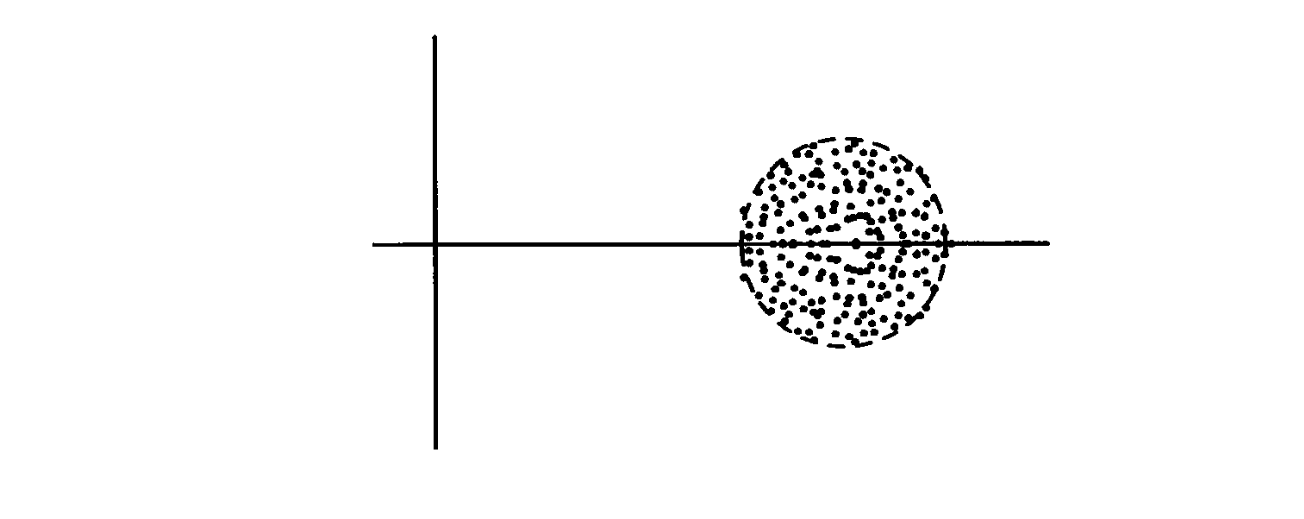
\includegraphics[width=0.8\textwidth]{figures/35-2.png}
\end{figure}
%────────────────────────────────────────
This figure shows the eigenvalues of $A$, a set of points roughly uniformly distributed in the disk of radius $1 / 2$ centered at $z=2$ .

Fig 34.1  shows the convergence curve for the GMRES iteration applied to the problem $A x=b$, where $b=(1,1, \ldots, 1)^*$. The convergence in this case is extraordinarily steady at a rate approximately $4^{-n}$. The reason for this is not hard to spot. Since the spectrum of $A$ approximately fills the disk indicated, $\|p(A)\|$ is approximately minimized by the choice $p(z)=(1-z / 2)^n$. Since $I-A / 2$ is a random matrix scaled so that its spectrum approximately fills the disk of radius $1 / 4$ about 0 , we have $\|p(A)\|=\left\|(I-A / 2)^n\right\| \approx 4^{-n}$. This matrix $A$ is well-conditioned, with condition number $\kappa(A) \approx 2.03$. The deviation from normality is modest, with $\kappa(V) \approx 141$. 

Figure 34.1 illustrates the convergence of matrix iterations under favorable circumstances-when the matrix $A$ is well behaved (which often means a good preconditioner has been applied). We see that six-digit accuracy is achieved after ten iterations, at a cost of approximately $10 \times 2 \mathrm{~m}^2=8.0 \times 10^5 \mathrm{flops}$, since the work is dominated by the matrix-vector multiplication at each step. Solving the same system by Gaussian elimination would require $\frac{2}{3} m^3 \approx 5.3 \times$ $10^6$ flops. This improvement by a factor close to 7 was achieved even though $A$ has no sparsity to take advantage of and even though the dimension $m=200$ is not high. For the same example with $m=2000$, GMRES would beat Gaussian elimination by a factor more like 70 . For a $2000 \times 2000$ matrix with similar spectral properties but $90 \%$ or $99 \%$ sparsity, the factor would improve to on the order of 700 or 7000 , respectively, and the storage required by GMRES would also diminish dramatically.
%────────────────────────────────────────
\begin{figure}[H]
    \centering
    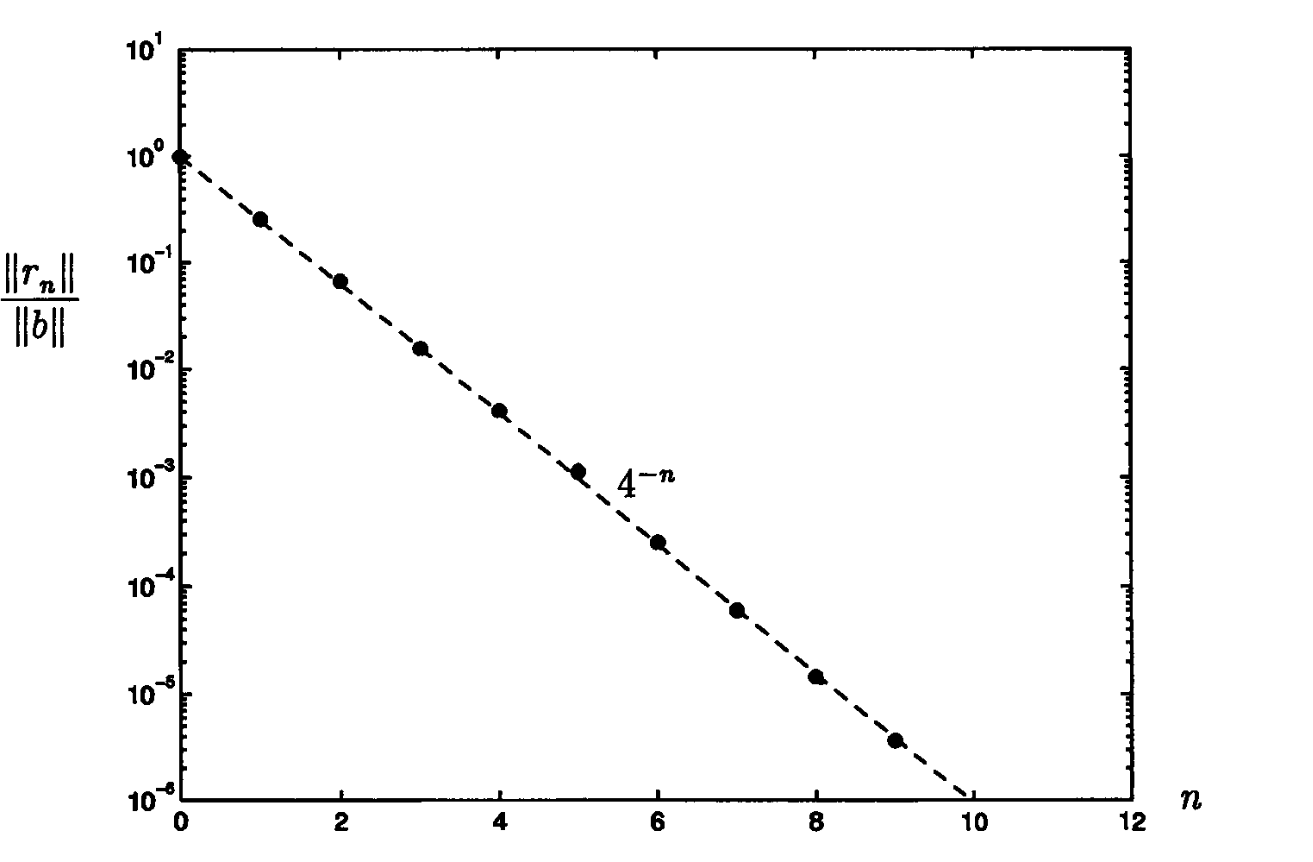
\includegraphics[width=0.8\textwidth]{figures/35-3.png}
    \caption{GMRES convergence curve for the same matrix A. This rapid, steady convergence is illustrative of Krylov subspace iterations under ideal circumstances, when $A$ is a well-behaved (or well-preconditioned) matrix.}
\end{figure}
%────────────────────────────────────────
\end{example}
%────────────────────────────────────────


%────────────────────────────────────────
\begin{example}
[A bad eg for GMRES]
\label{eg: A bad eg for GMRES}
If the eigenvalues of a matrix "surround the origin," on the other hand, such rapid convergence cannot be expected. Figures 35.4-35.5 present an example. The matrix is now $A^{\prime}=A+D$, where $A$ is the matrix of \eqref{eq: a good eg for GMRES} and $D$ is the diagonal matrix with complex entries
$$
d_k=\left(-2+2 \sin \theta_k\right)+i \cos \theta_k, \quad \theta_k=\frac{k \pi}{m-1}, 0 \leq k \leq m-1 .
$$

%────────────────────────────────────────
%────────────────────────────────────────
\begin{figure}[H]
\centering
\begin{minipage}{.5\textwidth}
  \centering
  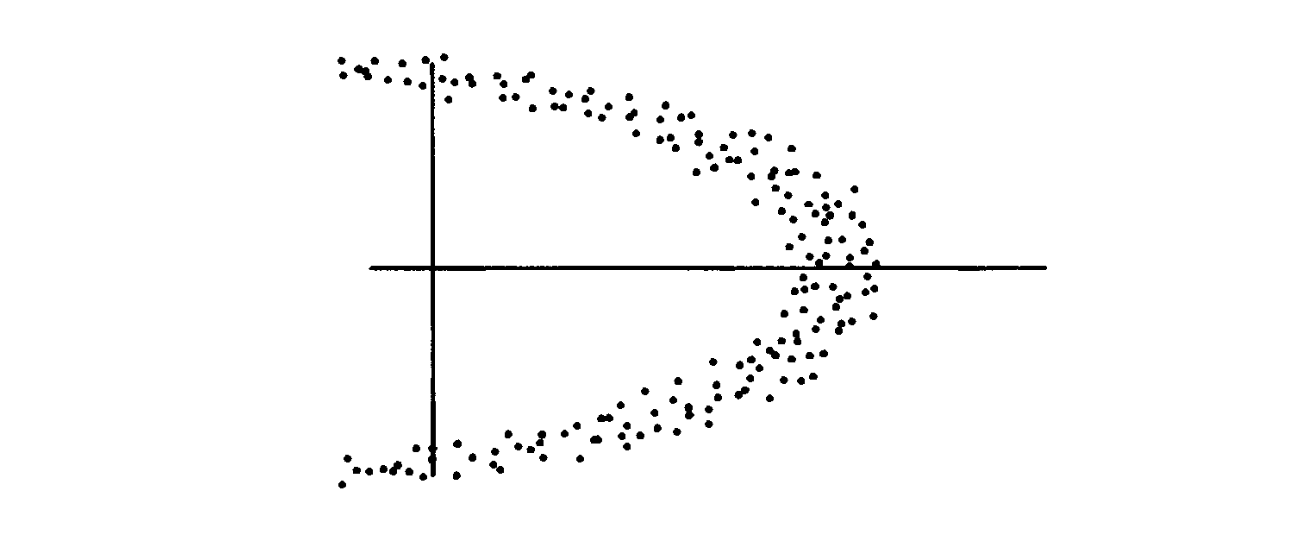
\includegraphics[width=.9\linewidth]{figures/35-4.png}

\end{minipage}%
\begin{minipage}{.5\textwidth}
  \centering
  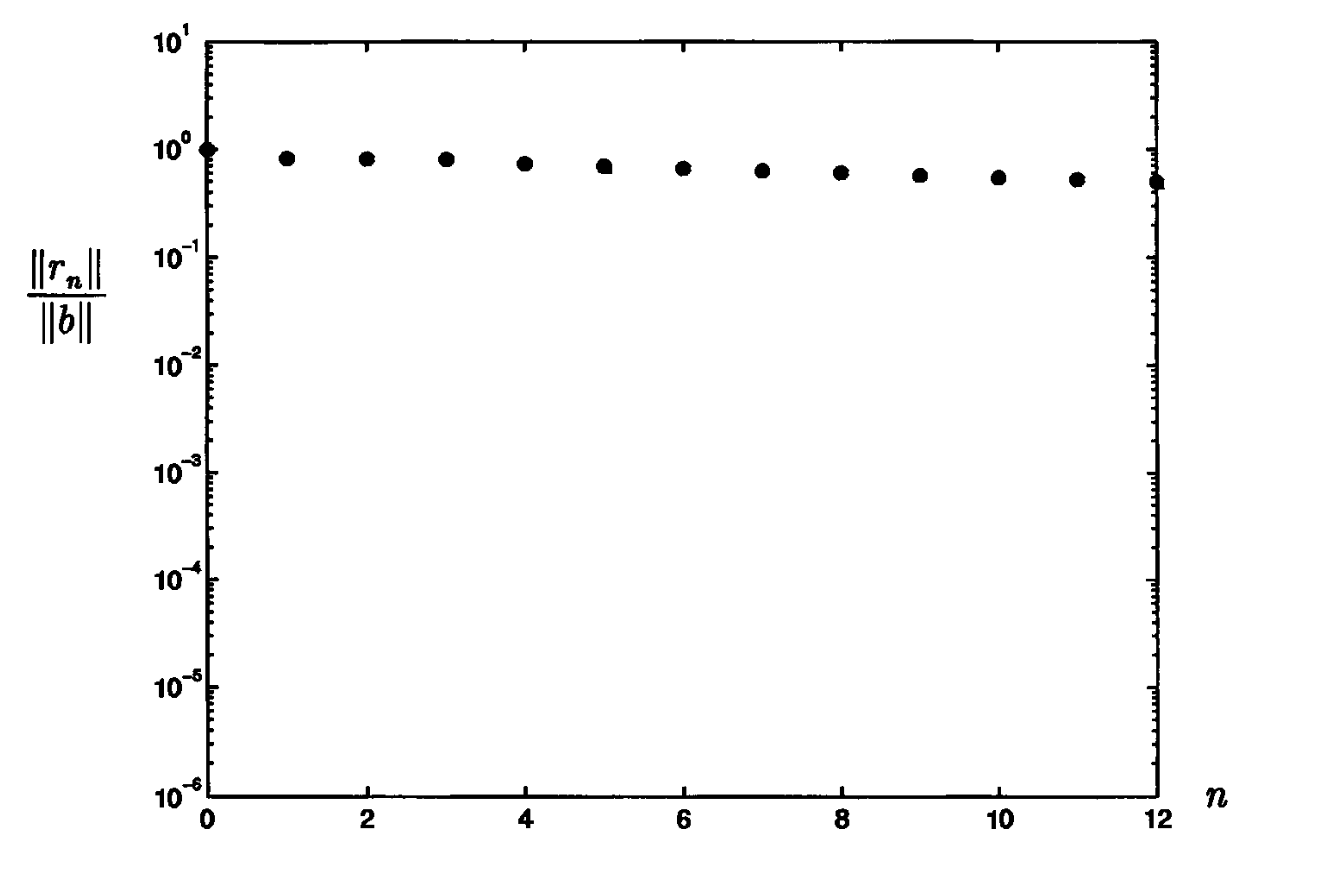
\includegraphics[width=.8\linewidth]{figures/35-5.png}

\end{minipage}
\end{figure}
%────────────────────────────────────────
%────────────────────────────────────────
As is evident in Figure, the eigenvalues now lie in a semicircular cloud that bends around the origin. The convergence rate is much worse than before, making the iterative computation no better than Gaussian elimination for this problem. The condition numbers are now $\kappa(A) \approx 4.32$ and $\kappa(V) \approx 54.0$, so the deterioration in convergence cannot be explained by conditioning alone; it is the locations of the eigenvalues, not their magnitudes (or those of the singular values) that are causing the trouble. If the arc extended much further around the spectrum, the convergence would worsen further.


\end{example}
%────────────────────────────────────────